\documentclass[10pt,a4paper]{article}
\usepackage[utf8]{inputenc}
\usepackage[english]{babel}
\usepackage{amsmath}
\usepackage{amsfonts}
\usepackage{amssymb}
\usepackage{graphicx}
\usepackage[left=2cm,right=2cm,top=2cm,bottom=2cm]{geometry}
\usepackage{mathtools}
\usepackage{xcolor}
\usepackage{booktabs}
\usepackage{verbatim}
\usepackage{float}
\usepackage{fancyhdr}
\usepackage{gensymb}
\usepackage{datetime}
\usepackage{verbatim}
\usepackage{enumerate}  
\usepackage{subcaption}
\usepackage{multicol}
\usepackage{cite}
\fancyhf{}
\renewcommand{\headrulewidth}{0pt}
\renewcommand \thesection {\Roman{section}}
\fancyfoot[L]{\today}
\fancyfoot[C]{\thepage}
\pagestyle{fancy}
\captionsetup{width=0.6\linewidth}

\begin{document}
\begin{center}
\huge{The influence of Temperature and a Lightguide on the Crosstalk Probability of a SiPM}\\ \vspace{0.8cm}
\large{Dominik Z\" urcher, dominikz@student.ethz.ch}\\ \vspace{0.2cm}
\large{Supervisors: }\\ 
\large{Prof. Adrian Biland, biland@phys.ethz.ch}\\ 
\large{Dominik Neise, neised@phys.ethz.ch}\\ 
\vspace{0.3cm}
\textit{Institute for Particle Physics and Astrophysics, Department of Physics, ETHZ}\\
\vspace{0.5cm}
\date{\today}                                           
\hrulefill \\
\textbf{Abstract} \\
\noindent
Silicon based photo multiplier promise to be a cost-efficient and robust alternative for classic photomultiplier tubes for many applications. An interesting property of such Silicon based photo multipliers is their optical crosstalk, where secondary photons originating from charge carrier avalanches might discharge neighboring cells. Therefore, the investigation of optical crosstalk is of major interest for those who want to use Silicon based photo multipliers for their needs. In this work the dependence of optical crosstalk on temperature and the usage of an acrylic glass lightguide was investigated using dark counts. The results indicate that the optical crosstalk increases with temperature. There are also indications that the use of a lightguide reduces the crosstalk probability, although this cannot be clearly answered due to large uncertainties. The results also show that the analysis performed in this work is insufficient. More events need to be recorded to decrease the uncertainties and the influence of the pulse selection has to be clarified before any clear statements about the influence of a lightguide can be made.
\end{center}
\hrulefill
\newpage
\setcounter{page}{1}
\begin{multicols}{2}
\section{Introduction}
One of the oldest and most popular methods for counting single photons is by the use of photomultiplier tubes (PMTs). Those devices which are typically combined with a lightguide are used in various disciplines where single photon detection is needed, such as elementary particle physics, medical diagnostics or spectroscopy. The combination of high gain and low noise as well as their large quantum efficiency makes PMTs the ideal candidates for those tasks \cite{Hama}. Unfortunately, PMTs show a so called \emph{aging} effect meaning that their properties such as quantum efficiency and gain change with age \cite{aging}. \\ \\ \noindent
A specific application of PMTs is their use in Imaging Air-Cherenkov telescopes used for the detection of very high energetic gamma ray sources. In such experiments the detectors are often exposed to strong background light such as star or moon light for a long time. Therefore, the PMTs used in the detector suffer from rapid aging and have to be replaced regularly, resulting in high costs \cite{gapd}. \\ \\ \noindent
A more robust alternative of photon detectors suitable for such experiments comes in the form of silicon based photo detectors composed out of multiple Geiger-mode avalanche photo diodes. Being the first telescope of its kind, the FACT telescope is pioneering this method since  its start of operation in 2011 \cite{fact}. \\ \\\noindent
A Geiger-mode avalanche photo diode (G-APD) consists out of a biased operated p-n junction. The applied bias voltage $V_A$ induces an electric field within the depletion layer of the junction. If the bias voltage is chosen above the breakdown voltage $V_B$ the electric field is large enough such that an electron-hole pair created by a single photon hitting the depletion layer results in a self-sustaining avalanche of charge carriers leading to a macroscopic current at the $\mu$A range. The breakdown voltage typically varies between 10 and a few 100 V depending on temperature and type of the G-APD. The performance of the G-APD depends strongly on the over voltage which is given by $V_E = V_A - V_B$. Especially gain and quantum efficiency of the G-APD strongly depend on it. Typically hundreds to a few thousand G-APD cells are combined into a single silicion photo multiplier (SiPM). \\ \\  \noindent
An important feature present in PMTs and SiPMs are the dark count events. Thermal excitations can lead to the production of avalanches even in the absence of illumination. In SiPMs the dark count rate increases with temperature and over voltage\cite{avalanche}. \\ \\  \noindent
An avalanche triggered by an external photon hitting one of the G-APD cells in an SiPM contains many secondary photons which may leak to a neighboring cell and trigger an avalanche there as well. This effect is regarded as optical crosstalk. Therefore, a single external photon may be counted as one, two or even more photons \cite{gapd}. Such events counting as one, two or three photons are further referred to as single photon events (SPE), double photon events (DPE) and triple photon events (TPE). \\ \\  \noindent
In this work the optical crosstalk properties of a SiPM similar to the ones used in the camera of the FACT telescope is studied. More specifically, it is investigated if the crosstalk probability depends on temperature and if it is affected by the use of an acrylic glass lightguide. This is done by investigating SPEs, DPEs and TPEs as measured in dark count events. See section 4 for more details.

\section{Methods}
The SiPM studied in this work is of the type MPPC S10362-33-100C and produced by Hamamatsu. The SiPM consists of 900 single G-APD cells covering an effective active area of 3x3 mm. The detector is designed to function within a temperature range from -20 to 40 $\degree$C and a bias voltage of 70 $\pm$ 10 V \cite{diode}. \\ \\  \noindent
Since the performance of the SiPM depends strongly on their temperature all measurements are performed in a C180 climate chamber by Weiss Technik \cite{schrank}. The temperature of the SiPM is monitored by a PT-1000 temperature sensor which is glued to the back of the SiPM directly. It was found that the experiment suffered from a lot of electronic noise. To reduce the noise all the hardware parts were connected to a common ground and the SiPM was placed in a Faraday cage. The experiments described in this work require the measurement of dark counts only. Therefore, a great effort was made to reduce the flux of external photons. To measure dark counts a continuous trigger was used to randomly record timelines with a sample rate of 2 GHz. \\ \\  \noindent
Spare parts of the FACT camera are used as readout electronics in order to simulate the conditions in the real telescope as close as possible. Also, the FACT software is used to readout the signal output of the SiPM. Figure 1 shows a rough schematic of the hardware used in the experiment. Some pictures of the used equipment are attached in the Appendix. The bias voltage was supplied by a power supply of Agilent Technologies of the type N5770A and monitored using a Solatron Schlumberger 7081 precision voltmeter.
\end{multicols}
\begin{figure*}
\centering

\includegraphics[width= 7cm]{circuit2}
\caption{Schematic of the readout electronics.}
\label{fig1} 
\end{figure*}
\begin{multicols}{2}
\subsection{Breakdown Voltage Measurement}
In order to study the crosstalk properties of the SiPM the breakdown voltage of the used SiPM has to be known. This is needed since the operation performance of the SiPM depends on the choice of the over voltage. Since the breakdown voltage depends strongly on temperature one would have to measure it at each temperature separately. Fortunately, for the SiPM in question a linear behavior of the breakdown voltage with temperature has been shown. The linear law has a dependence of 55 mV/K which is the same for every SiPM of this kind \cite{gapd}. Therefore, the knowledge of the breakdown voltage at a certain temperature is enough. The absolute values of the breakdown voltage vary from SiPM to SIPM depending on fabrication. The breakdown voltage was determined experimentally at a temperature of 25 $\degree$C. The determination of the breakdown voltage can be done by measuring the gain of the SiPM at different bias voltages. The gain was determined at six different voltages in the range from 69.3 to 70.5 V. At each of the different voltages 10'000 randomly triggered timelines were recorded. See section 4 for further details on how the breakdown voltage was calculated.

\subsection{Temperature Dependence Measurement}
Two properties of optical crosstalk are investigated in this work:
\begin{itemize}
\item dependence on temperature
\item influence of an acrylic glass lightguide
\end{itemize} 
To investigate those properties 30'000 randomly triggered timelines were recorded each at 5 different temperatures ranging from 5 $\degree$C to 25 $\degree$C. The temperature range was chosen according to the temperatures measured in the camera of the FACT telescope during its operation \cite{fact}. The bias voltage was adjusted with temperature in order to achieve a constant over voltage and therefore a similar performance of the SiPM at each measurement. In addition to changing the temperature each measurement has been performed twice, once without a lightguide and once with an acrylic glass lightguide. The lightguides used in this work are the same which were also used in the design of the original FACT camera. To avoid unwanted effects by unknown optical properties of glue, the lightguide has not been glued onto the SiPM but was fixed onto it using optical grease. 

\section{Results}

\subsection{Determination of Breakdown Voltage}
In order to determine the breakdown voltage of the investigated SiPM the gain was measured at six different bias voltages. The breakdown voltage is defined as the bias voltage where the gain of the SiPM reaches zero. This point is estimated by fitting a linear function of the form
\begin{equation}
g = s \cdot (V_A-V_B)
\end{equation}
to the data where $s$ indicates the change of the gain with over voltage. The collected data points are given in Table 1. Figure 2 shows the resulting graph. The obtained values for $s$ and the breakdown voltage are given in Table 2. \\ \\  \noindent 
According to Hamamatsu the breakdown voltage might vary from SiPM to SiPM. Unfortunately, the sheet listing the breakdown voltage of the specific SiPM investigated here was no longer available. Therefore, it is not possible to make any estimates about the precision of this method. However, one can state that it is in the voltage range indicated by Hamamatsu.

\end{multicols}
\begin{figure}[H]
\centering
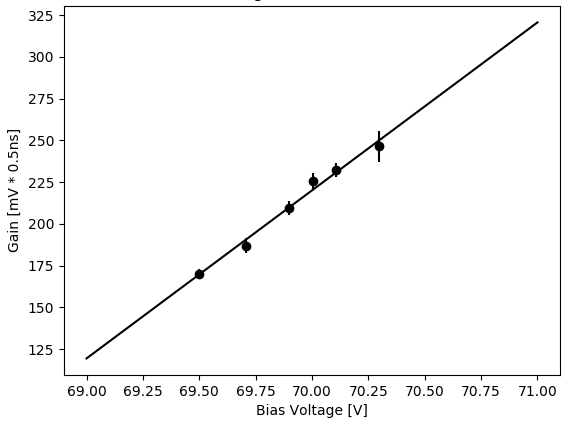
\includegraphics[width=10cm]{Breakdown}
\caption{Display of the data used to determine the breakdown voltage of the SiPM. The solid black line indicates the linear fit.}
\label{fig3}
\end{figure}

\begin{table}[H]
\centering
\caption{Data used for the determination of the breakdown voltage.}
\begin{tabular}{|c|c|}
\hline 
Bias Voltage [V] & Gain [mV 0.5ns] \\ 
\hline 
69.497 & 170 $\pm$ 2.816 \\ 
\hline 
69.706 & 187 $\pm$ 4.440 \\ 
\hline 
69.900 & 210 $\pm$ 4.271\\ 
\hline 
70.004 & 226 $\pm$ 5.120\\ 
\hline 
70.105 & 232 $\pm$ 4.476\\ 
\hline 
70.295 & 246 $\pm$ 9.210\\ 
\hline 
\end{tabular} 
\label{Table 1}
\end{table}
\begin{table}[H]
\centering
\caption{Fitting parameters obtained in the breakdown voltage measurement.}
\begin{tabular}{|c|c|}
\hline 
 $s$ [0.0005 ns]  & $V_B$ [V] \\ 
\hline 
101 $\pm$ 5.594 & 67.8 $\pm$ 0.117 \\ 
\hline 
\end{tabular} 
\label{Table 2}
\end{table}
\begin{multicols}{2}
\subsection{Temperature Dependence Measurement}
After determination of the breakdown voltage of the SiPM the over voltage was chosen as 2.4 V. An increase in the over voltage evidently leads to a higher gain making the pulses larger and more visible. On the other hand, the noise is increased at the same time. Choosing the best suited over voltage is therefore a trade off and depends on the noise properties of the experiment in question. Empirically 2.4 V was found to be a suitable choice for this experiment. Table 3 summariezes the results of the measurements. As one can learn from Table 3, the bias voltage has been changed in accordance with the change in temperature in order to keep the over voltage and therefore the performance of the SiPM at a constant level. Figure 3 displays the change of the crosstalk probability with temperature as well as the influence of a light guidance. The fitting parameters of the two linear fits displayed in Figure 3 are given in Table 4 where $C_0$ indicates the crosstalk probability at 0 $\degree$C and $s$ the differential change in crosstalk probability with respect to change in temperature. \\ \\ \noindent
From the inspection of Figure 3 one can learn that the crosstalk shows a clear increase with temperature. This is also in agreement with the results of A. Biland et al., where a weak temperature dependence was found \cite{gapd}. Notice that in the work of A. Biland et al. a crosstalk probability of the order of 12$\%$ was found whereas a probability around 45$\%$ is stated in this work. This is reasonable since A. Biland et al. operated their G-APDs at an over voltage of 1.4 V whereas an over voltage of 2.4 V is used in this work increasing the magnitude of the crosstalk probability. However, note that other investigations lead to different conclusions. As an example, no temperature dependence was found by \cite{crossref}. So far there is no theoretical model available favoring any of the two dependencies. \\ \\  \noindent
One can also learn that the usage of a lightguide seems to decrease the crosstalk probability equally at all temperatures.
Such an effect was expected considering that the complex shape of the lightguide could cause thermal photons to be scattered multiple times and leaving the lightguide more easily. One should point out that the uncertainties in Figure 3 are too large at the time being and no clear statement about the influence of the lightguide can be made. In the scope of this work it was also realized that the method by which the events are selected from the timeline strongly influences the results. There is no clear answer to how one should select them.
\end{multicols}
\begin{figure}[H]
\centering
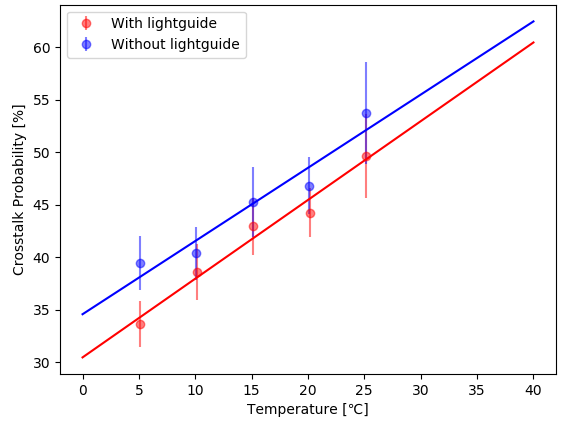
\includegraphics[width=10cm]{crosstalkplot}
\caption{Display of the data showing how the crosstalk probability changes with temperature and by the use of a lightguide.}
\label{fig3}
\end{figure}
\begin{table}[H]
\centering
\caption{Data used in the crosstalk probability investigation.}
\begin{tabular}{|c|c|c|c|c|}
\hline 
Voltage [V] & Temperature [$\degree$C] & Crosstalk [\%] & Gain [mV 0.5ns] & Dark count rate [MHz] \\ 
\hline 
 \multicolumn{5}{|l|}{Without light guidance} \\ 
\hline 
69.097 & 5 & 40 $\pm$ 2.560 & 248 $\pm$ 2.655 &  12.0 $\pm$ 0.433\\ 
\hline 
69.382 & 10 & 40 $\pm$ 2.540 & 250 $\pm$ 2.590 & 16.3 $\pm$ 0.565\\ 
\hline 
69.710 & 15 & 45 $\pm$ 3.327 & 250 $\pm$ 2.874 & 22.5 $\pm$ 0.823\\ 
\hline 
69.920 & 20 & 47 $\pm$ 2.698 & 237 $\pm$ 2.124 & 24.8 $\pm$ 0.693\\ 
\hline 
70.202 & 25 & 54 $\pm$ 4.846 & 228 $\pm$ 2.740 & 14.6 $\pm$ 0.560\\ 
\hline 
 \multicolumn{5}{|l|}{With light guidance} \\ 
\hline 
69.010 & 5 & 34 $\pm$ 2.209 & 235 $\pm$ 2.729 & 9.4 $\pm$ 0.323\\ 
\hline 
69.383 & 10 & 39 $\pm$ 2.697 & 249 $\pm$ 2.881 & 9.5 $\pm$ 0.364\\ 
\hline 
69.710 & 15 & 43 $\pm$ 2.713 & 252 $\pm$ 2.510 & 22.4 $\pm$ 0.731\\ 
\hline 
69.918 & 20 & 44 $\pm$ 2.359 & 237 $\pm$ 2.002 & 24.5 $\pm$ 0.657\\ 
\hline 
70.199 & 25 & 50 $\pm$ 3.985 & 230 $\pm$ 2.656 & 15.2 $\pm$ 0.562\\ 
\hline 
\end{tabular} 
\label{Table 3}
\end{table}
\begin{table}[H]
\centering
\caption{Fitting parameters obtained in the crosstalk measurement.}
\begin{tabular}{|c|c|}
\hline 
 \multicolumn{2}{|l|}{Without light guidance} \\ 
\hline 
$C_0$ [\%] & $s$ [\% K$^{-1}$] \\ 
\hline 
30 $\pm$ 1.191 & 0.75 $\pm$ 0.0712 \\ 
\hline 
 \multicolumn{2}{|l|}{With light guidance} \\ 
\hline 
$C_0$ [\%] & $s$ [\% K$^{-1}$] \\ 
\hline 
35 $\pm$ 1.817 & 0.7 $\pm$ 0.109 \\ 
\hline 
\end{tabular} 
\label{Table 4}
\end{table}
\begin{multicols}{2} \noindent
In order to investigate the consistency of the measurements the gain and the dark count rate were monitored alongside the crosstalk probability as well. As mentioned before, the over voltage has to be adjusted with temperature in order to achieve a constant gain for all the measurements. Figure 4 shows the gain measured at the different temperatures. One can observe that it is rather constant with a maximal fluctuation of 20 $mV \cdot 0.5ns$. In order to explain the measured variation of the crosstalk probability (say a 5\% change) one would require a change in the gain of 100 mV at the very least \cite{hamaref}. Therefore, the change of the crosstalk probability cannot be explained by the fluctuations in the gain. \\ \\ \noindent
A. Biland et al. propose a change of the dark count rate of approximately 0.225 MHz per temperature change of one Kelvin, whereas Figure 5 indicates a change of approximately 0.833 MHz per Kelvin \cite{gapd}. A possible explanation for this discrepancy might be the difference in cell size of the used G-APD. The G-APDs used by A. Biland et al. are four times smaller leading to a lower fill factor \cite{diode}. Therefore, the SiPM used in this work covers a larger area with G-APD cells and it is natural to assume that more area leads to a larger rate change with temperature. Note that the last point in Figure 5 does not follow the general trend which is probably caused by the selection algorithm becoming inefficient at this point. At 25 $\degree$C the dark count rate becomes so large that events are happening very shortly after each other and most of them are therefore disregarded by the algorithm. See section 4 for further information. \\ \\ \noindent
In the end one can state that the measurements taken are reasonable and the increase of the crosstalk probability with temperature cannot be regarded as an artifact caused by fluctuations of the measurement parameters.
\end{multicols}
\begin{figure}
\centering
\begin{minipage}{.5\textwidth}
  \centering
  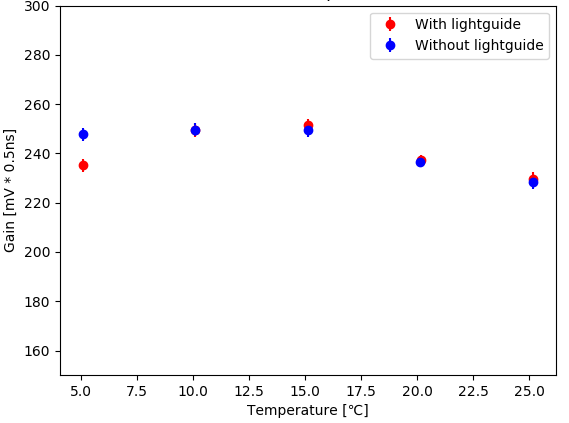
\includegraphics[width=\linewidth]{gainplot}
  \captionof{figure}{Visualization of the gain measurements taken along the crosstalk measurements.}
  \label{fig2}
\end{minipage}%
\begin{minipage}{.5\textwidth}
  \centering
  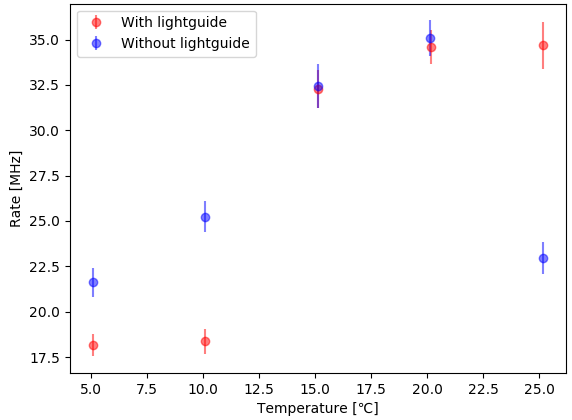
\includegraphics[width=\linewidth]{rateplot}
  \captionof{figure}{Dark count rates measured during the crosstalk measurements.}
  \label{fig3}
\end{minipage}
\end{figure}
\begin{multicols}{2}
\section{Analysis}
The readout software of the FACT camera outputs the recorded signal in the zFits format which is a specific format used by the FACT collaboration \cite{zfitspaper}. The conversion into normal data arrays can be done using a readout tool which is accessible on github \cite{zFits}. The software used for the analysis of the data in this work is also publicly available on github \cite{software}. The analysis can be roughly divided into three parts for each measurement point: 
\begin{enumerate}[(i)]
\item Search the recorded timelines for photon events 
\item Integrate over those events to differentiate SPE, DPE and so on
\item Make a histogram and extract gain and crosstalk probability from it
\end{enumerate}
Step (i): An example timeline can be seen in Figure 6. The voltage is binned in 1024 bins each having a length of 0.5 ns. In Figure 6 the shape of a typical photon event can be seen. Such events show a very characteristic steep rising edge and a rather slowly falling edge. Higher photon events like DPE, TPE and so on posses the same characteristic shape as the SPE but they have a larger amplitude. In addition to the searched for dark count signals one also records signals caused by noise, the most problematic one being ringing events as shown in Figure 7. Generally influence of the noise increases as the temperature is raised. Due to the presence of the noise a stable algorithm to search for photon events is needed. Following the example of \cite{singlephoton} a convolution of the timeline with a kernel of the analytic form 
\begin{equation}
V=A \cdot (1- \exp{(-B \cdot t)}) \cdot \exp{(-C \cdot t)},
\end{equation}
which resembles the actual signal shape, is performed giving more weight to kernel-shaped events. In the above equation $A$, $B$, $C$ are coefficients and $t$ and $V$ indicate time and voltage respectively. Such a convolved signal is shown in Figure 8. Subsequently, a numerical derivative of the convolved timeline is taken to search for the characteristic steep rising edges of the dark count events. In order to be considered as a valid photon event the rising edge must also have a minimal amplitude. A complication is added in the form of photon events happening shortly after each other as seen in Figure 9. Such events should not be counted as a DPE since they are not caused by optical crosstalk. In order to avoid counting such events as a DPE an additional condition is implied: If two events happen shortly after each other the first one is not considered but only the second one sitting on top of the first one. Also, in order to perform a proper integration there must not be any event shortly after the event in consideration. Therefore, in the end only stand alone events or events sitting on top of other events are considered in the analysis.\\  \\  \noindent
Step (ii): The integration over the selected events is performed numerically using the composite trapezoidal rule. However, the final value of the integral has to be corrected for the variation of the zero line. This is especially important if the considered signal is sitting on top of another event. To do so, the zero line is approximated performing an interpolation between the minimum in front of the signal and the end of the signal as can be seen in Figure 10. The obtained integrals are of the units mV $\cdot$ 0.5 ns and represent the charge released by the charge carrier avalanches in the G-APD cells. One expects that a DPE triggering two avalanches at once results in approximately double the amount of charge released in a SPE and therefore also in double size of the integral.\\  \\  \noindent
Step (iii): The integral values collected within all the events belonging to a certain measurement point are summarized in a histogram. In the best case one can already spot by eye the peaks belonging to the SPE, DPE and even TPE. The gain measuring the charge released by the avalanche triggered by a single photon can be obtained by forming the difference of the position of the first and second or also between the second and third peak. The crosstalk probability measuring the ratio between multiple photon events (DPE, TPE) and the total number of events can be obtained by estimating the total amount of SPEs, DPEs and TPEs recorded. This is done by fitting the sum of three normal distributions to the histogram and measuring their areas as indicated in Figure 11.
\end{multicols}
\begin{figure}
\centering
\begin{minipage}{.5\textwidth}
  \centering
  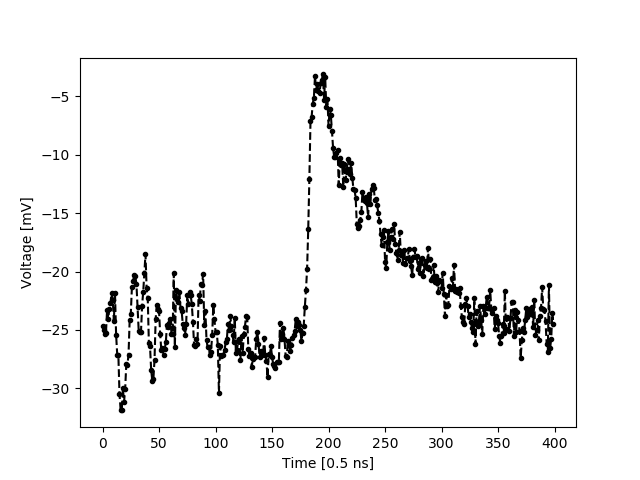
\includegraphics[width=\linewidth]{peak}
  \captionof{figure}{A characteristic signal shape of a photon event as measured in the experiment before any manipulation is performed.}
  \label{fig2}
\end{minipage}%
\begin{minipage}{.5\textwidth}
  \centering
  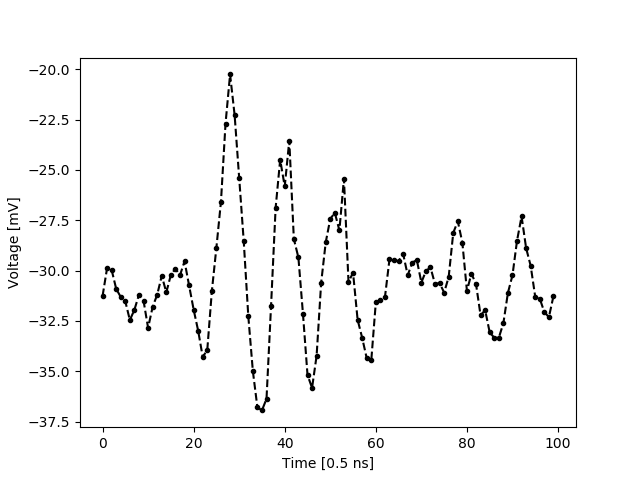
\includegraphics[width=\linewidth]{ringing}
  \captionof{figure}{Problematic ringing noise event. The signal contains many steep raising edges although there is no dark count event present.}
  \label{fig3}
\end{minipage}
\end{figure}

\begin{figure}
\centering
\begin{minipage}{.5\textwidth}
  \centering
  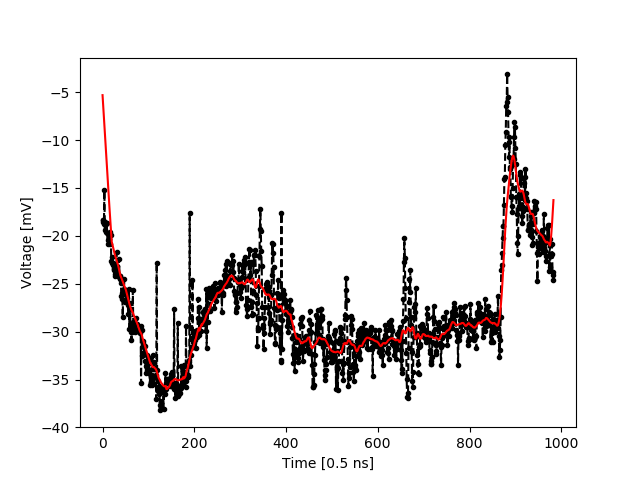
\includegraphics[width=\linewidth]{convolved}
  \captionof{figure}{In black is the original timeline containing a lot of noise. The red line indicates the timeline after convolution. Notice that the noise is greatly reduced.}
  \label{fig4}
\end{minipage}%
\begin{minipage}{.5\textwidth}
  \centering
  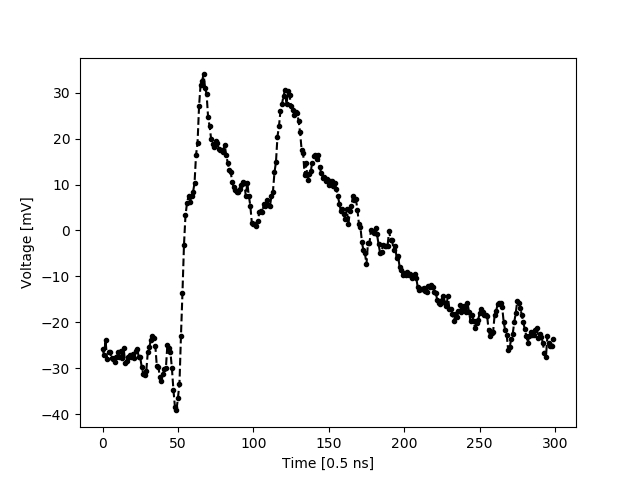
\includegraphics[width=\linewidth]{double}
  \captionof{figure}{Two photon events happening shortly after each other. Naive integration would lead to a large integration area interpreted as a DPE.}
  \label{fig5}
\end{minipage}
\end{figure}

\begin{figure}
\centering
\begin{minipage}{.5\textwidth}
  \centering
  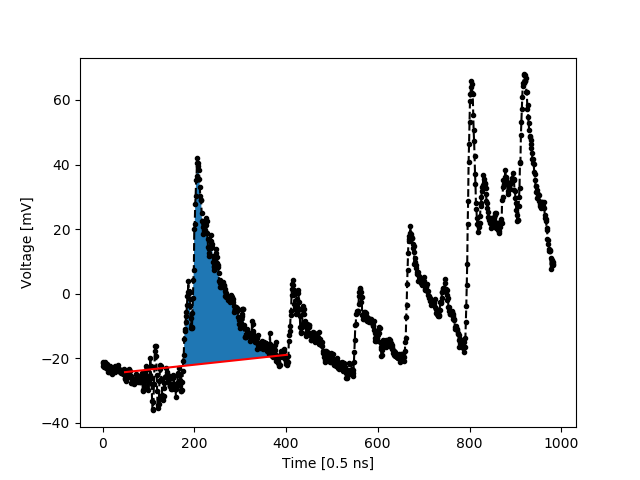
\includegraphics[width=\linewidth]{integration}
  \captionof{figure}{The red line indicates the interpolation of the zero line, whereas the blue area marks the resulting area of the peak.}
  \label{fig6}
\end{minipage}%
\begin{minipage}{.5\textwidth}
  \centering
  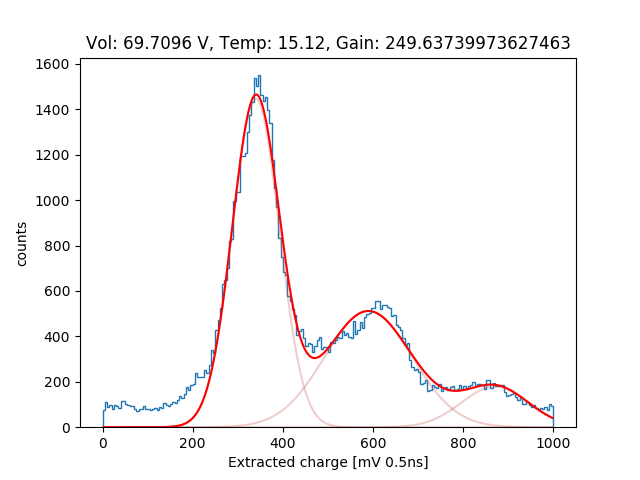
\includegraphics[width=\linewidth]{fingerplot}
  \captionof{figure}{Visualisation of a histogram. The shown histogram includes all the events recorded at a temperature of 20 $\degree$C. The light red curves indicate the three normal distributions describing the individual peaks. The solid red line displays their sum which has been fitted to the histogram.}
  \label{fig7}
\end{minipage}
\end{figure}
\newpage
\begin{multicols}{2}
\section{Conclusion and Outlook}
The scaling behavior of the crosstalk probability with temperature found in this work is in agreement with the results of A. Biland et al. but disagrees with the work of T. Krähenbühl. There are indications, that the usage of a lightguide leads to a reduction of the crosstalk probability. However, it was also found that the amount of data collected is not enough to allow to clearly answer this question. In following works aiming at answering this question more data should be analyzed. One should also try to reduce the noise in the experiment. Empirically, it was found that the algorithm which selects the events which are taken into account for the analysis greatly influences the outcome and interpretation of the results. It is proposed that one should test the algorithm using known events from a simulation in order to find the most suitable method. A simulation explaining the influence of a lightguide would also be helpful for the interpretation of the data. At last, one should notice that the type of SiPM investigated here is known to show natural inhomogeneities due to fabrication and multiple SiPMs should be investigated instead of only one.
\end{multicols}
\section{Appendix}
\begin{figure}[H]
\centering
\begin{minipage}{.5\textwidth}
  \centering
  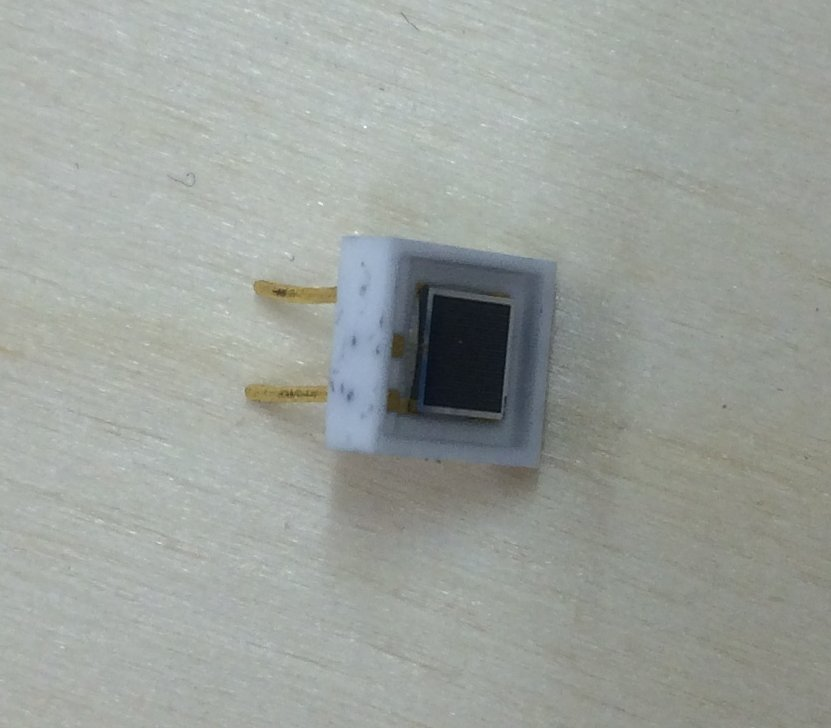
\includegraphics[width=0.9\linewidth]{diode.JPG}
  \captionof{figure}{The SiPM of the type MPPC S10362-33-100C which was investigated.}
  \label{fig2}
\end{minipage}%
\begin{minipage}{.5\textwidth}
  \centering
  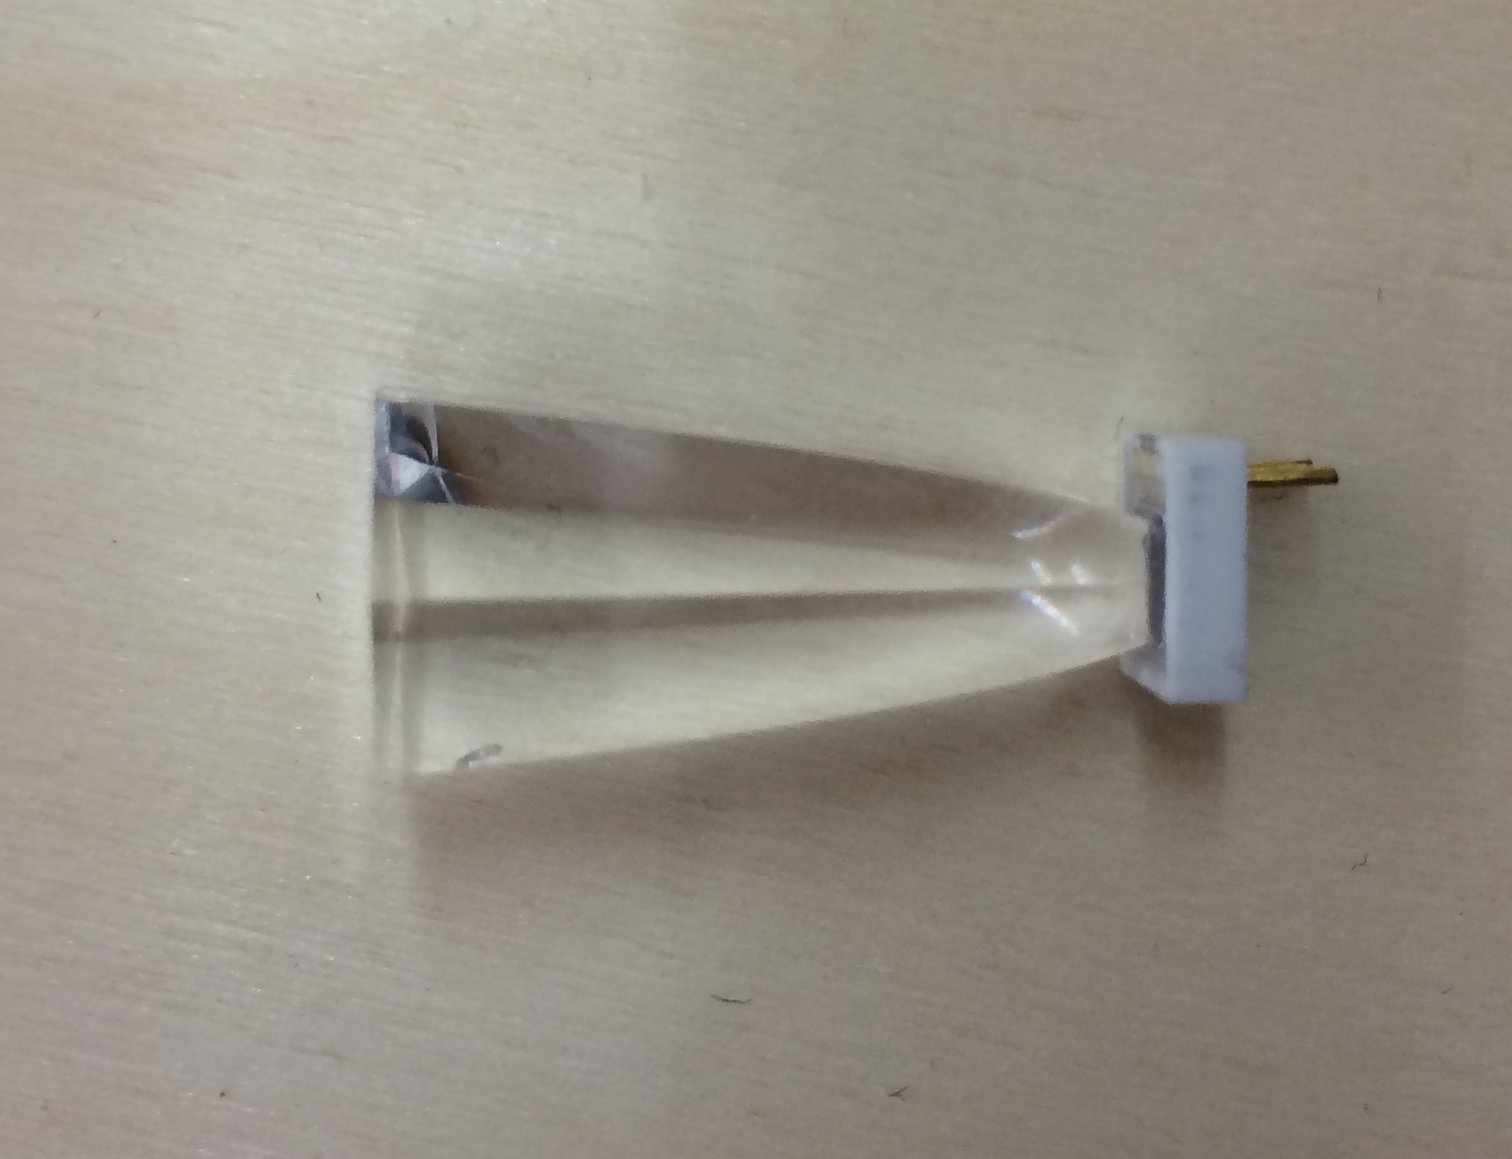
\includegraphics[width=0.9\linewidth]{cone.JPG}
  \captionof{figure}{The investigated SiPM with the lightguide fixed to it.}
  \label{fig3}
\end{minipage}
\end{figure}

\begin{figure}[H]
\centering
\begin{minipage}{.5\textwidth}
  \centering
  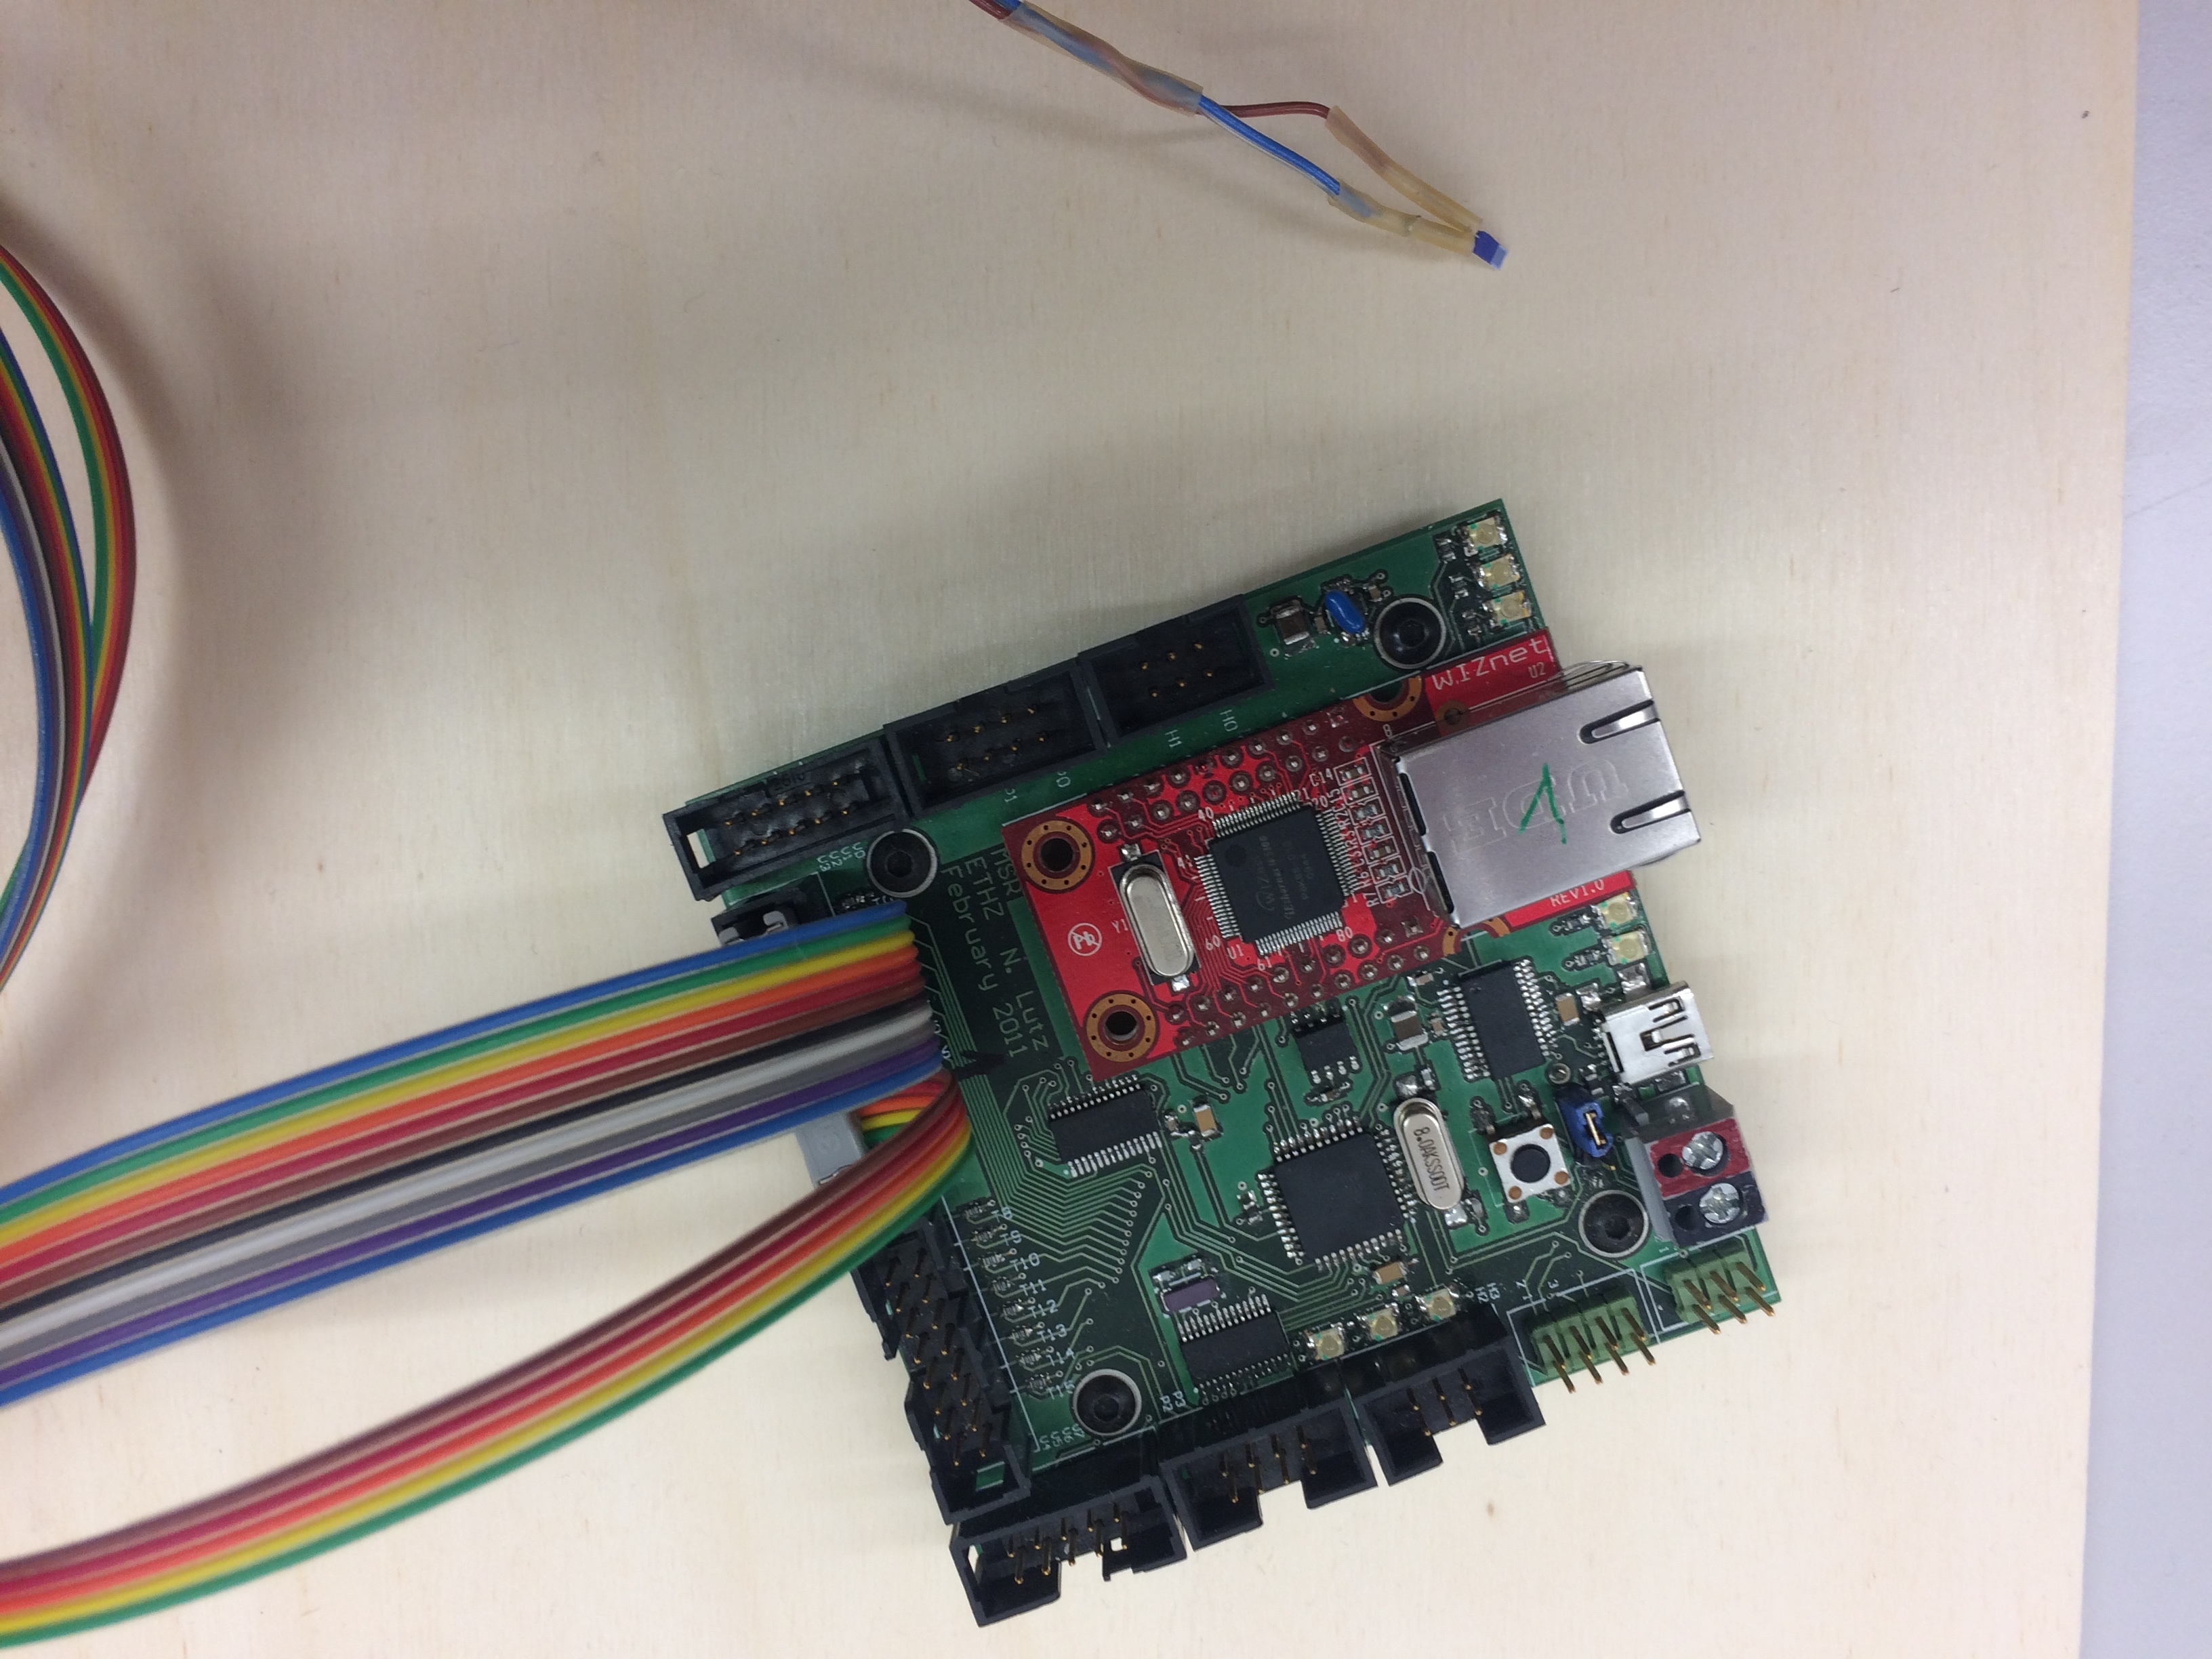
\includegraphics[width=0.9\linewidth]{MSR.jpg}
  \captionof{figure}{The MSR module used for the readout of the PT-100 temperature sensors including one of the sensors.}
  \label{fig4}
\end{minipage}%
\begin{minipage}{.5\textwidth}
  \centering
  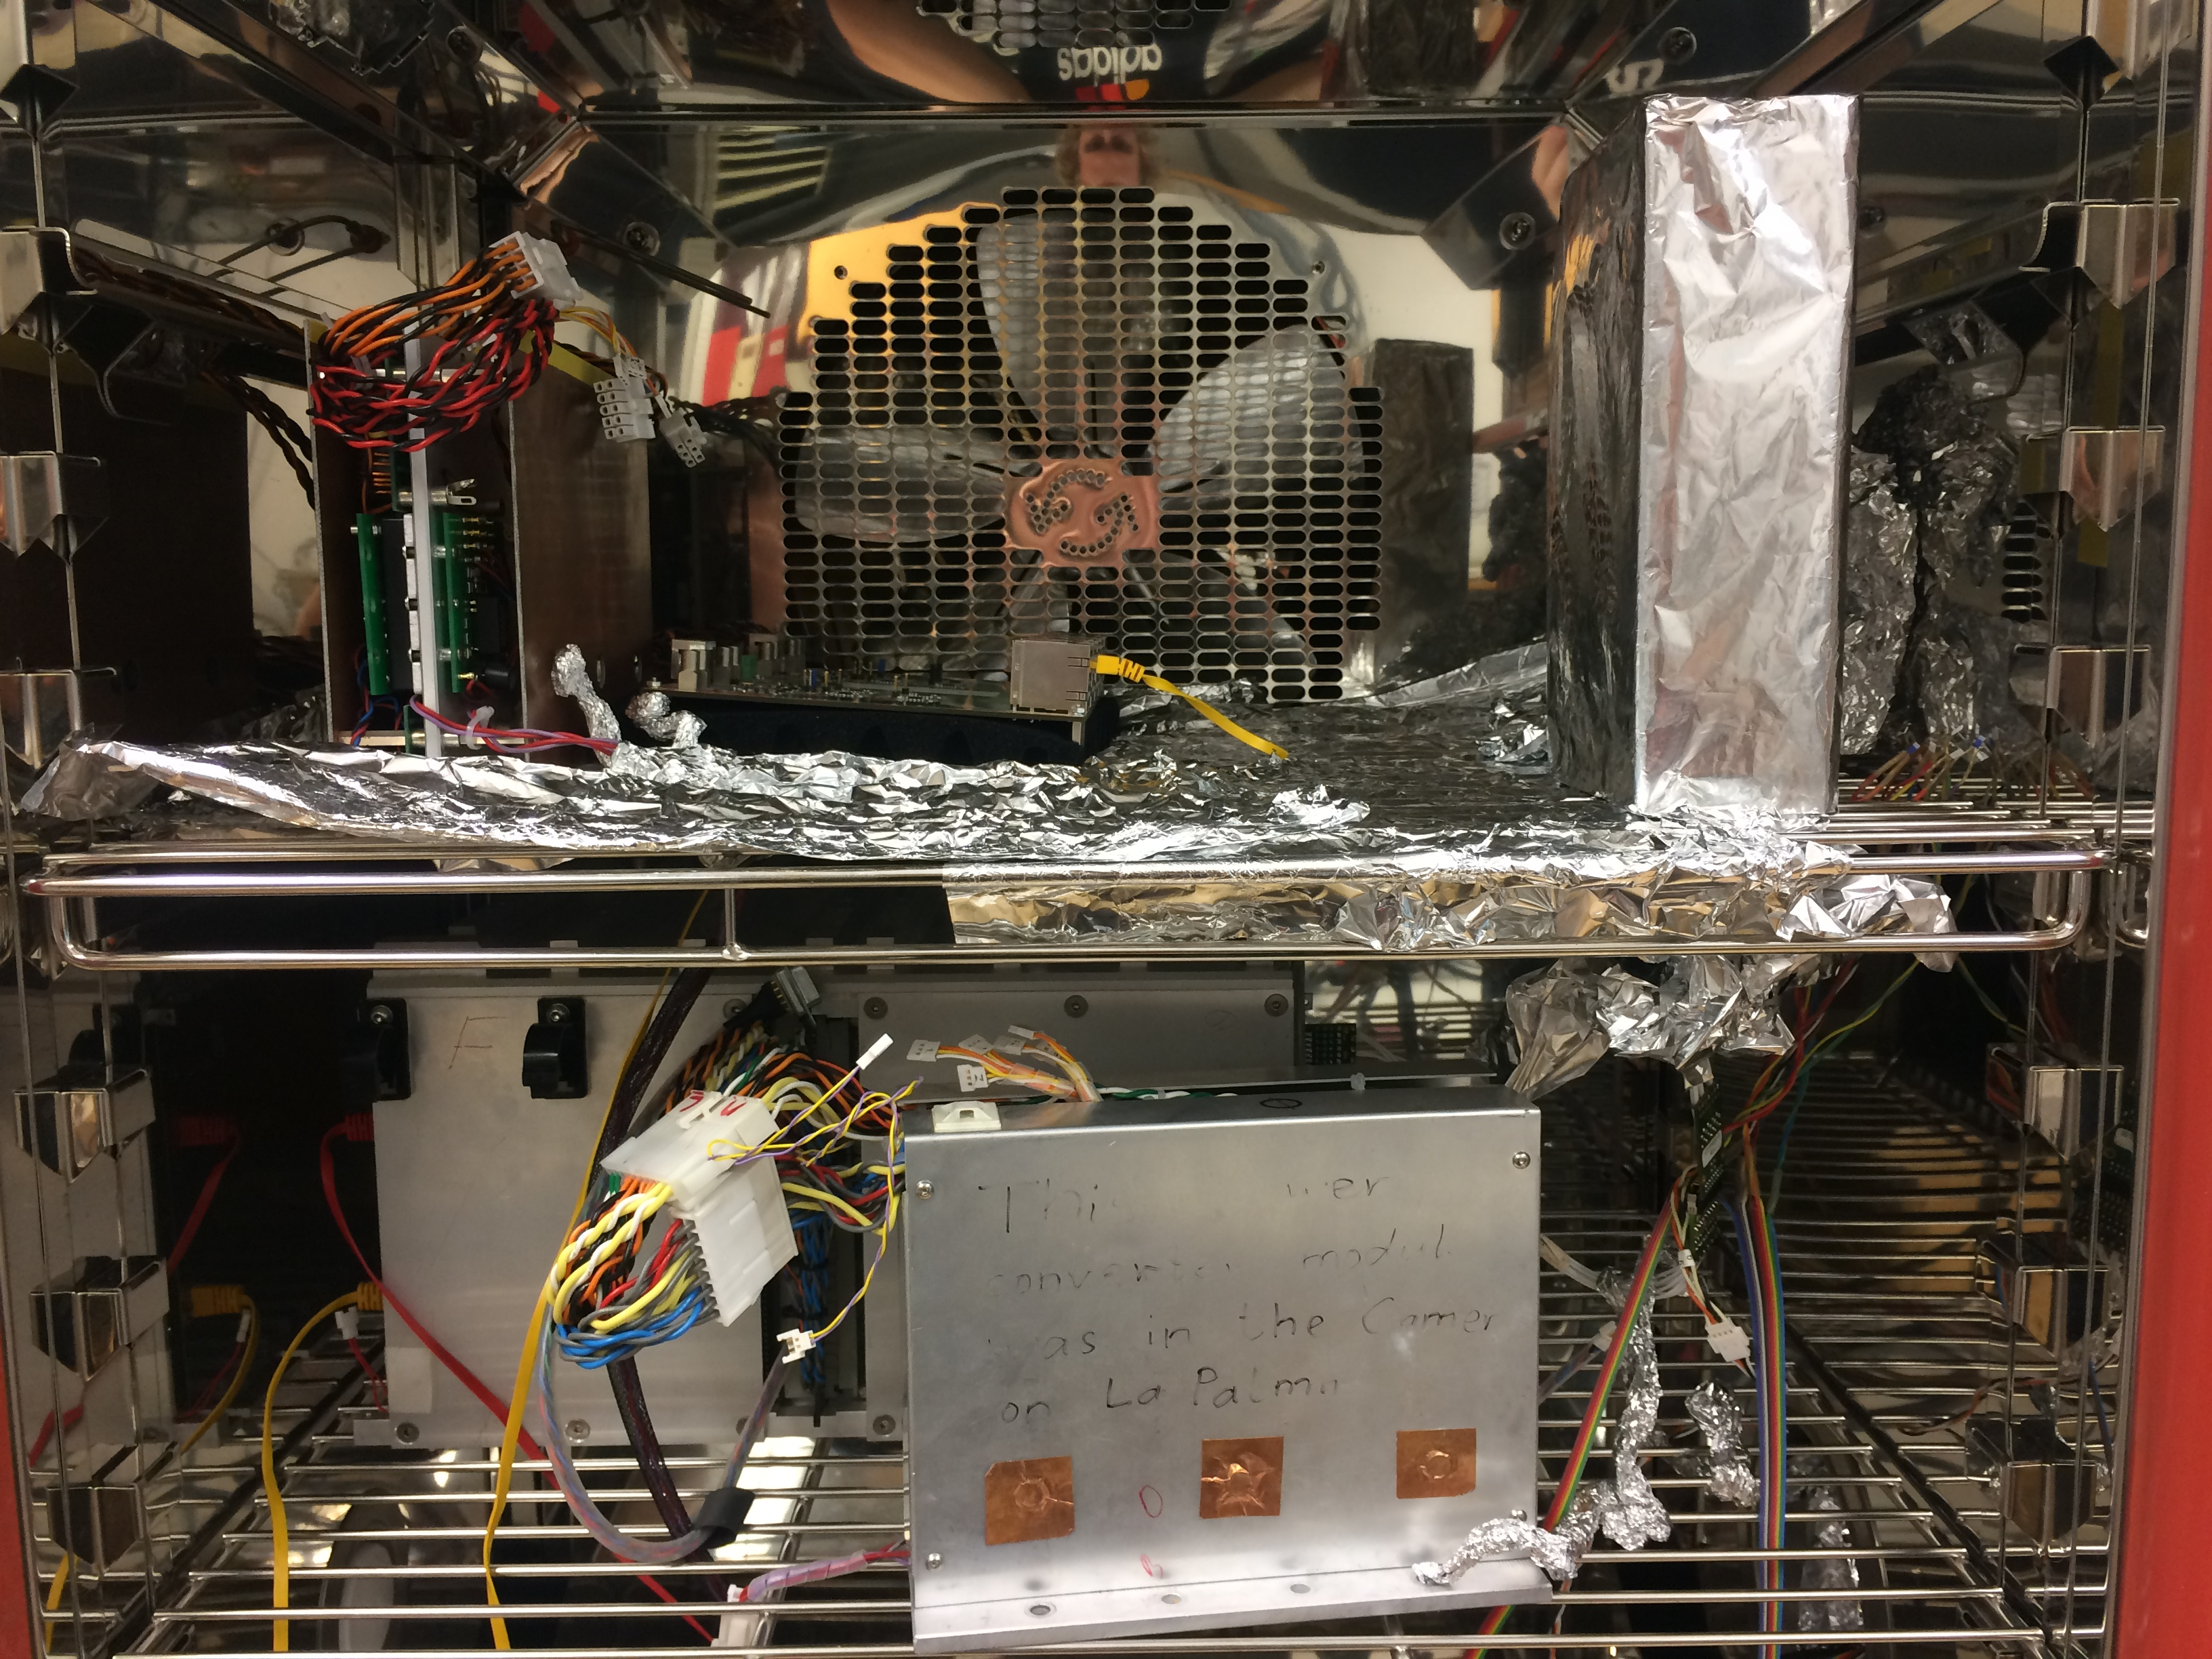
\includegraphics[width=0.9\linewidth]{equipement.JPG}
  \captionof{figure}{Full setup of the hardware within the climate chamber as used for the measurements.}
  \label{fig5}
\end{minipage}
\end{figure}
\newpage

\bibliography{Library}{}
\bibliographystyle{IEEEtran}

\end{document}